% Chapter 5

\chapter{Analytical and Experimental Results} % Main chapter title

\label{Chapter5} % For referencing the chapter elsewhere, use \ref{Chapter1} 

\lhead{Chapter 5. \emph{Analysis and Conclusion}} % This is for the header on each page - perhaps a shortened title

%----------------------------------------------------------------------------------------
\section{Fourier Analysis}
\label{Fourier}
One of the most pressing concerns regarding switching power supplies is the spectral content of the output signal, both before and after filtering. This is of chief concern to power systems designers because the demands that excess spectral content can place on filtering increase size, weight, and cost of the inverter system. These additional frequencies represent energy that must be dissipated by the filter, and hence an inefficiency in our system. A comparative analysis of the dominant PWM techniques is necessary to understand the costs and benefits of each technique, but more importantly for the purpose of this paper, to understand how the hybrid algorithm used to modulate pulse-widths stacks up. In this section we lean heavily on the work of Zhous in \cite{FourierAnalysis}. We contribute to this discussion by analyzing the performance of closed loop control, where Zhou strictly examines open loop PWM inverters.

Recall that any signal can be decomposed into a sum of sines and cosines given by the expression:
\begin{equation}
f_N(\omega t) = \frac{a_0}{2} + \sum_{n=1}^N \left(\overbrace{a_n}^{A_n \sin(\phi_n)} \cos(n\omega t) + \overbrace{b_n}^{A_n \cos(\phi_n)} \sin(n\omega t)\right)\\
= \sum_{n=-N}^N c_n\cdot e^{in\omega t}
\end{equation}

Where
\begin{align*}
& ~~~~~ a_0 = \frac{1}{T}\int_{0}^{T}f(t)dt \\
a_n &= \frac{2}{T}\int_{t_0}^{t_0+T} f(t)\cdot  \cos(n\omega t)\ dt \\
b_n &= \frac{2}{T}\int_{t_0}^{t_0+T} f(t)\cdot  \sin(n\omega t)\ dt \\
c_n &= \frac{1}{T}\int_{t_0}^{t_0+T} f(t)\cdot e^{-in\omega t}\ dt
\end{align*}

\begin{equation}
c_n \ \stackrel{\mathrm{def}}{=} \ \begin{cases}
\frac{A_n}{2i} e^{i\phi_n} = \frac{1}{2}(a_n - i b_n) & \text{for } n > 0 \\
\frac{1}{2}a_0 & \text{for }n = 0\\
c_{|n|}^*  & \text{for } n < 0.
\end{cases}
\end{equation}


The magnitude of every harmonic of the fundamental can be found by:

\begin{align*}
K_0 &= \frac{a_0}{2} \\
K_n &= \sqrt{a_n^2+b_n^2}
\end{align*}

Note that in all cases it is understood that $n\in \mathbb{Z}$.

Additionally, because direct application of the Fourier analysis can be cumbersome, the analysis of less friendly waveforms can be simplified by the application of the following properties of symmetry.

For \textbf{odd symmetry}, that is, functions satisfying the equality $f(t)=-f(-t)$ it is given that:
\begin{equation}
\begin{cases}
a_n = 0 \\ 
b_n = \frac{2}{\pi}\int_{0}^{\pi}f(\omega t)\sin(n\omega t)d\omega t
\end{cases}
\end{equation}

For \textbf{half-wave symmetry}:
\begin{equation} 
\begin{cases} 
C_n = 0 &\mbox{for even n}  \\ 
a_n = \frac{2}{\pi}\int_{0}^{\pi}f(\omega t)\cos(n\omega t)d\omega t &\mbox{for odd n}  \\
b_n = \frac{2}{\pi}\int_{0}^{\pi}f(\omega t)\sin(n\omega t)d\omega t &\mbox{for odd n} 
\end{cases}
\end{equation}

This condition holds when $f{\omega t} = -f(-\omega t + \frac{T}{2})$.

And for \textbf{quarter-wave symmetry}:
\begin{equation} 
\begin{cases} 
a_0 = 0 \\
a_n = 0 &\mbox{for even n}  \\
a_n = \frac{8}{T}\int_{0}^{\frac{T}{4}}\cos{n\omega t} &\mbox{for odd n}  \\
b_n = 0 &\mbox{for all n} 
\end{cases}
\end{equation}
Quarter-wave symmetry holds for signals possessing half-wave symmetry, and also symmetry about the midpoint of the positive and negative half cycles.

\subsection{Total Harmonic Distortion and Electromagnetic Interferance}
One of the most common metrics for assessing the quality of a signal is the total harmonic distortion (THD.) The THD is given by the expression:
\begin{equation}
THD=\frac{\sqrt{\sum_{2}^{\infty}(V_n^2)_{rms}}}{(V_1)_{rms}} = \frac{(V)_{rms}^2-(V_1)^2_{rms}}{(V_1)_{rms}} = \frac{\sqrt{K_0^2+K_1^2+\ldots+K_n^2}}{K_1}\cdot100\%
\end{equation} 
`Where ${V_n}_{rms}$ is the rms value of the $n^{th}$ harmonic of $V_0(t)$, while ${V_1}_{rms}$ is the rms value of the fundamental frequency component.'\cite{FourierAnalysis} The ideal to which we strive is a zero value for THD; however, this is typically unattainable in a real-world inverter implementation. As one of the primary metrics used to assess the spectral content of a signal, we aim to minimize the THD seen at the output of an inverter. With the Fourier series, we are able to derive the expected THD analytically for

By using Fourier series, the determination of THD of a certain output is easy to obtain because magnitude of each harmonic $(C_n)$ can be calculated.

From Maxwell's equations, we know that quickly varying electric fields cause the propogation of electromagantic transverse waves. This phenomena is commonly reffered to as electromagnetic interference (EMI). This radiated energy can couple into adjacent circuits and interfere with sensitive circuitry. Ostensibly, this noise can also couple into the inverter itself and introduce noise into analog measurements critical for operation of feedback loops. The Federal Communications Commision (FCC) has strict guidelines regarding the level of radiated energy allowable by any particular electronic device. FCC Part 15 B, concerning unintentional radiators, is the section we are most concerned with.  The FCC guidelines dictate that power inverters do not generate excessive harmonic content or EMI, that inverters should be immune to other sources of EMI, and that the level of EMI generated by any inverter does not interfere with the normal operation of surrounding devices. 

Although these concerns are generally beyond the scope of this research, it is still an area of critical research to evaluate where the hybrid approach stands with respect to other PWM methods for its assessment as a product in the future. Because we have no plans for grid-tie capability at this time, we omit a coverage of common mode `series' filtering in this paper.

For the following subsections, we will refer to the switching pairs (Q1, Q2) and (Q3, Q4) as shown in the H-bridge in Figure \ref{hBridge}.

\begin{figure}
\centering
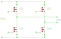
\includegraphics[width = 3.5in]{hBridge}
\caption{The H-bridge circuit showing switching-leg pairs (Q1, Q2) and (Q3, Q4)}, and opposing-leg pairs (Q1, Q4) and (Q2, Q3)
\label{hBridge}
\end{figure}


\subsection{Analyzing the Spectrum of Bipolar PWM}
The operation of a bipolar switching scheme generally operates as follows:
\begin{equation}
\begin{cases}
\label{bipolarStates}
V_{out} = V_{dc} &\mbox{if $V_{ref} > V_{c}$} \\
V_{out} = -V_{dc} &\mbox{if $V_{ref} < V_{c}$}
\end{cases}
\end{equation}

In this inversion scheme, opposing switching pairs are modulated simulataneously. 
Where $V_{ref}$ is the reference signal, and $V_c$ is the carrier signal. In Figure \ref{bipolarSwitchingOperation} we can see that $V_{out} = V_{AO}-V_{BO}$ resulting in an output that exists only in one of the two states described in equation \ref{bipolarStates}. If we select an odd modulation index, the output waveform exhibits odd-symetry and we can effectively eliminate all even harmonics at the output.

\begin{figure}
\centering
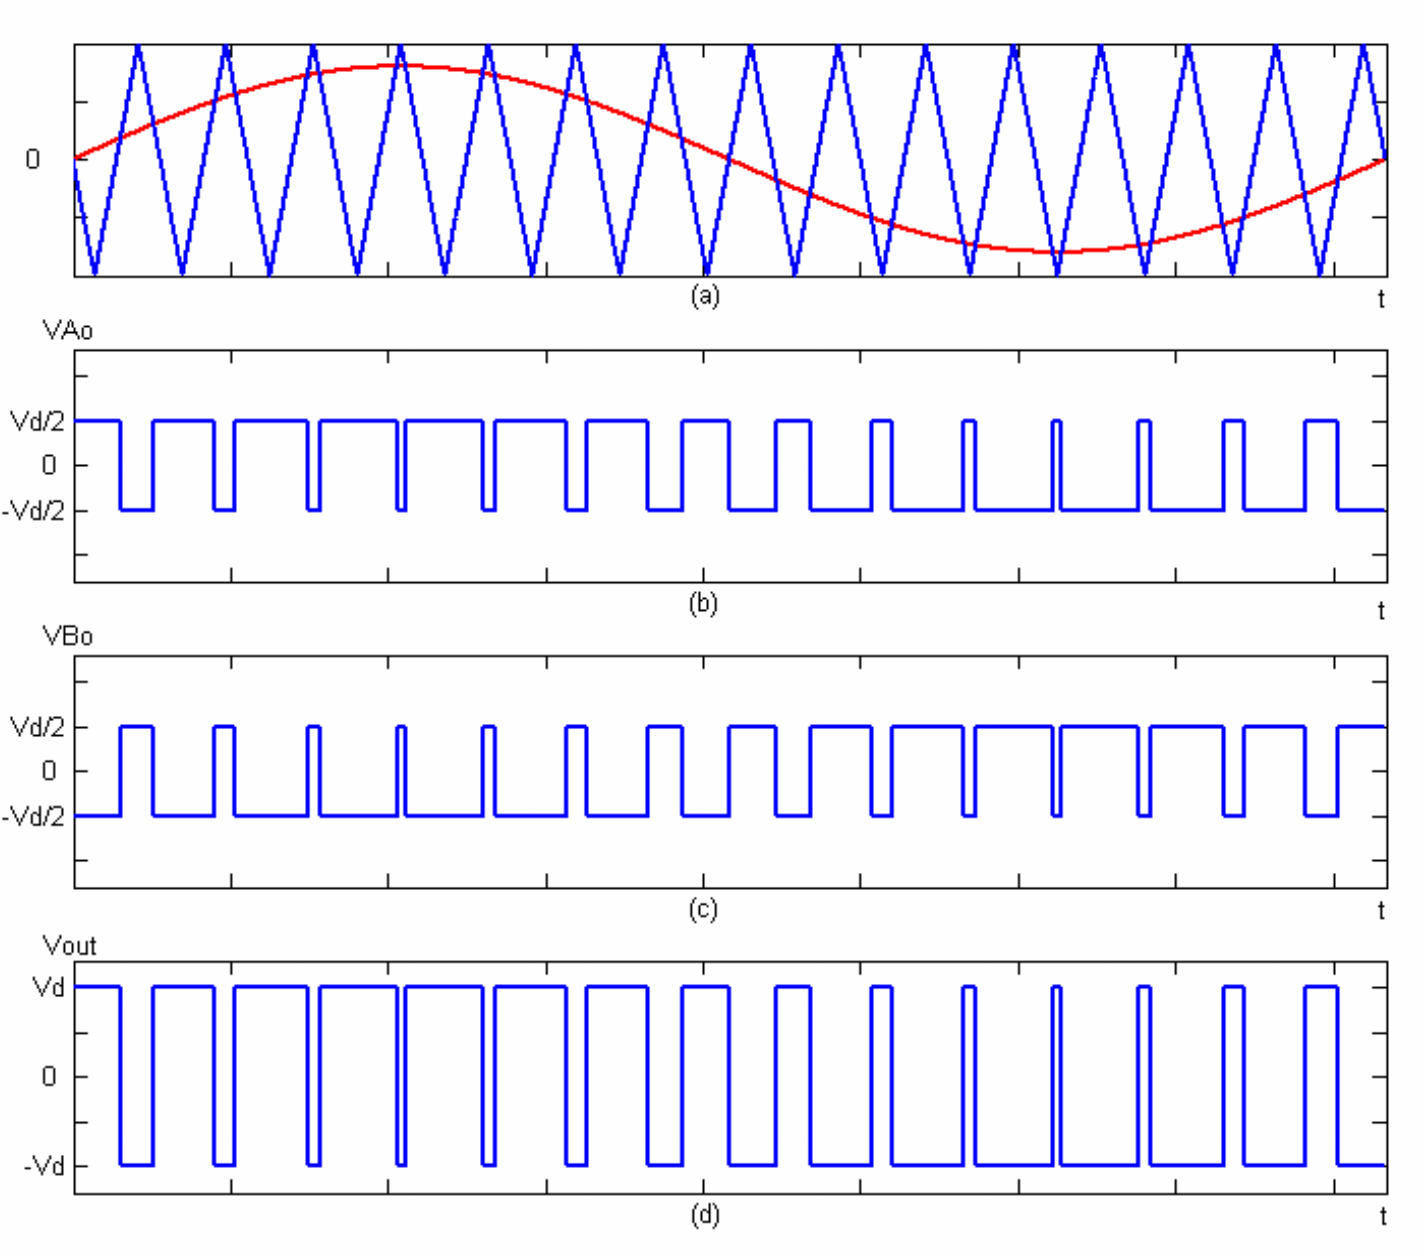
\includegraphics[width = 3.5in]{bipolarPwmShot}
\caption{The operation of a bipolar switching scheme for an inverter.\cite{FourierAnalysis}} 
\label{bipolarSwitchingOperation}
\end{figure}

In Simulink we implemented a simple bipolar inverter and performed an FFT using the powerGUI in SimPower Systems. The results are shown in Figure \ref{bipolarFFTMatlab}. The THD of this signal is found to be nearly $147\%$, and we note that the harmonics at the the frequency of modulation are greater than the fundamentals for this scheme.

\begin{figure}
\centering
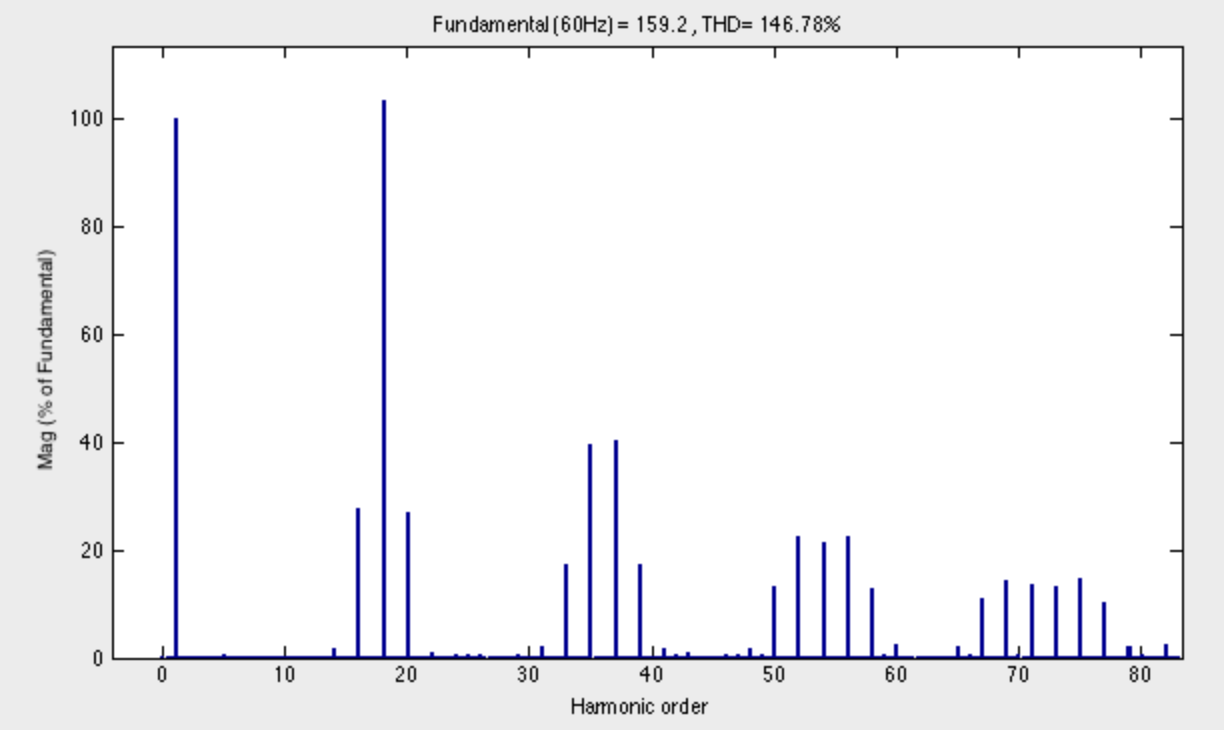
\includegraphics[width = 3.5in]{bipolarFFTMatlab}
\caption{The spectral content of a bipolar inverter is given by FFT, with harmonics shown as multiples of the fundamental at 60Hz}
\label{bipolarFFTMatlab}
\end{figure}

Analytically, from \cite{FourierAnlaysis}, we get that the Fourier coefficients of the bipolar switching scheme are:

\begin{equation}
a_n = \frac{2}{\pi} \Big[\int_{\theta_1}^{\theta_2} \cos(n\omega t) d\omega t + \int_{\theta_2}^{\theta_3} -\cos(n\omega t)d\omega t +\ldots +
\int_{\theta_{k-1}}^{\theta_{k}} (-1)^k \cos(n\omega t)d\omega \Big]
\end{equation} 
and 
\begin{equation}
b_n = \frac{2}{\pi} \Big[\int_{\theta_1}^{\theta_2} \sin(n\omega t) d\omega t + \int_{\theta_1}^{\theta_2} -\sin(n\omega t)d\omega t +\ldots +
\int_{\theta_{k-1}}^{\theta_{k}} (-1)^k \sin(n\omega t)d\omega t \Big]
\end{equation} 

Due to time constraints, we were not able to perform analyses on a bipolar inverter in hardware; the focus of this work is on the industry standard unipolar scheme discussed in the next subsection. 

\subsection{Analyzing the Spectrum of Unipolar PWM}
\label{uniSpectrum}
The operation of the unipolar PWM works under the following rules, given a triangular carrier signal and a sinusoidal reference. Note that in Figure \ref{unipolarStates}, ${V_{control}}_{1}$ is the dual of ${V_{control}}_{2}$, so we only require a single control signal in software.

\begin{equation}
\label{unipolarStates}
\begin{cases}
V_{out} = V_{dc} &\mbox{if $V_{ref} > V_{c}$}  \\
V_{out} = -V_{dc} &\mbox{if $V_{ref} < V_{c}$}  \\
V_{out} = 0 &\mbox{if $V_{ref} < V_{c}$}  \\
\end{cases}
\end{equation}

From this control law, one obtains the resultant waveforms shown in Figure \ref{unipolarPwmShot}.
\begin{figure}
\centering
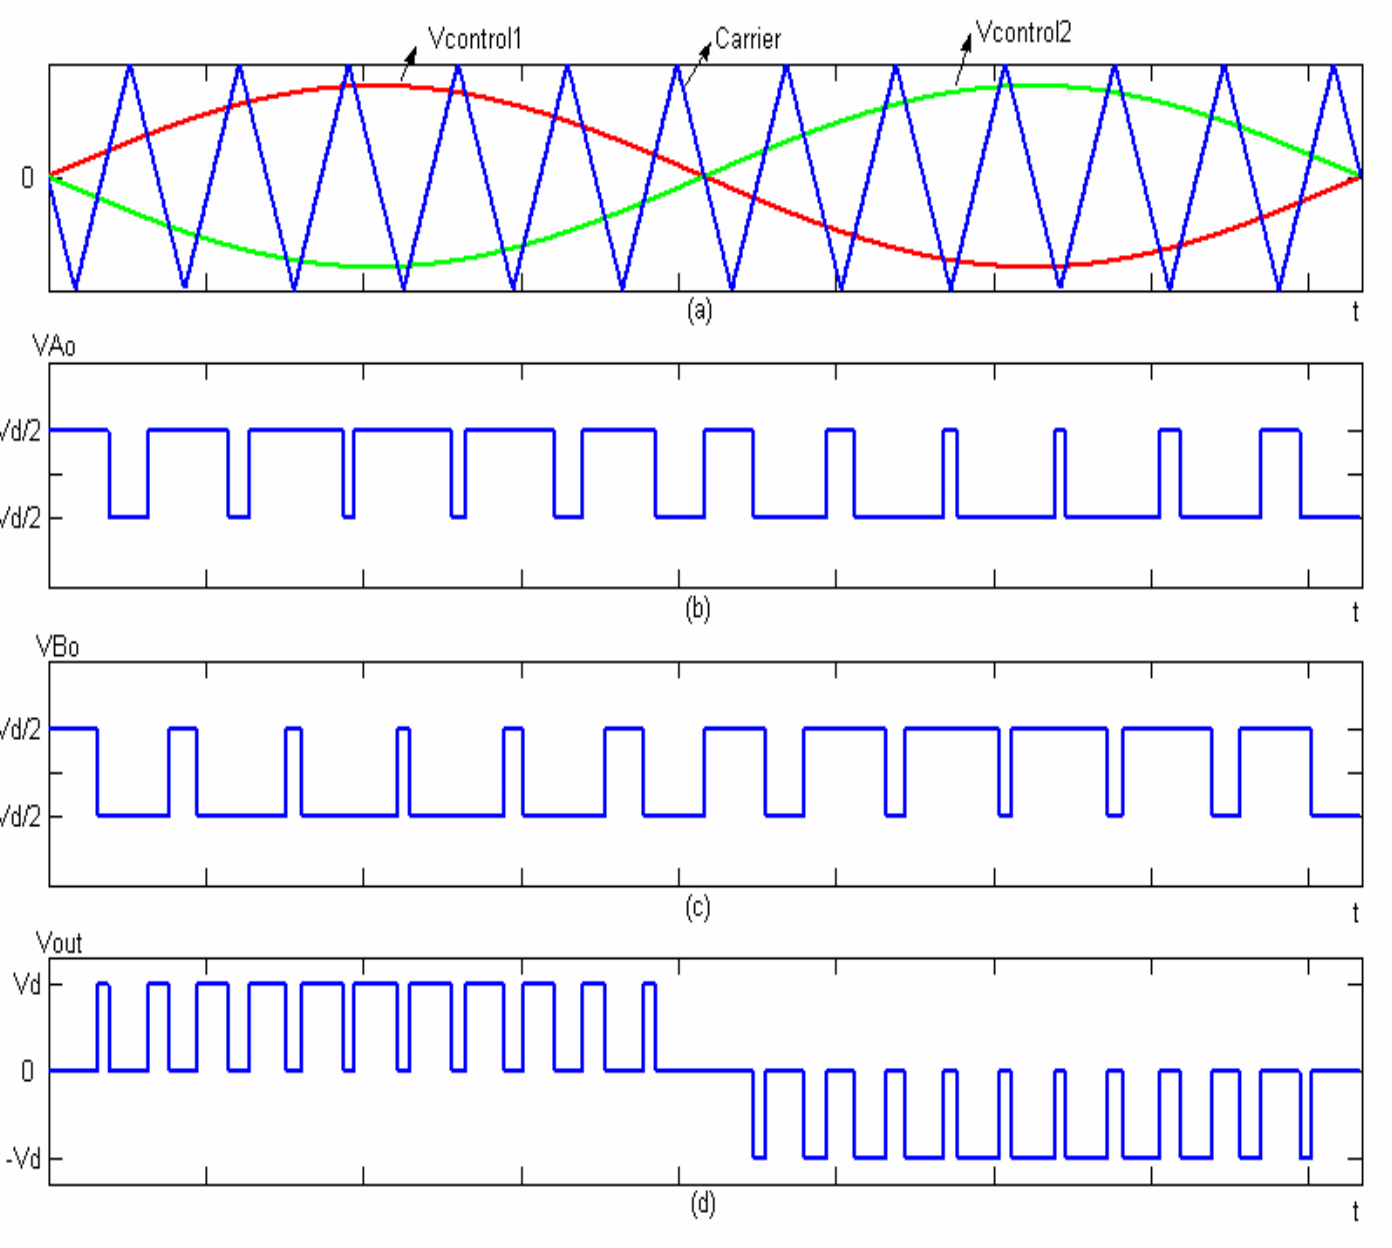
\includegraphics[width = 3.5in]{unipolarPwmShot}
\caption{The operation of a unipolar switching scheme for an inverter. Note that a single control signal is used in our software implementation since each control signal is the other's dual. \cite{FourierAnalysis}}
\label{unipolarPwmShot}
\end{figure}

Again, using Simulink we implemented a unipolar inverter and performed an FFT using the powerGUI in SimPower Systems. The results are shown in Figure \ref{unipolarFFTMatlab}. The THD of this signal is found to be around $77\%$, or nearly half that of the bipolar scheme. Here, the magnitdude of the fundamental is greater than any of the harmonics. These results confirm those of \cite{FourierAnalysis}, though we found the THD of the bipolar scheme in our simulation to be much higher. Both measurements were taken before any kind of filtering stage. 

\begin{figure}
\centering
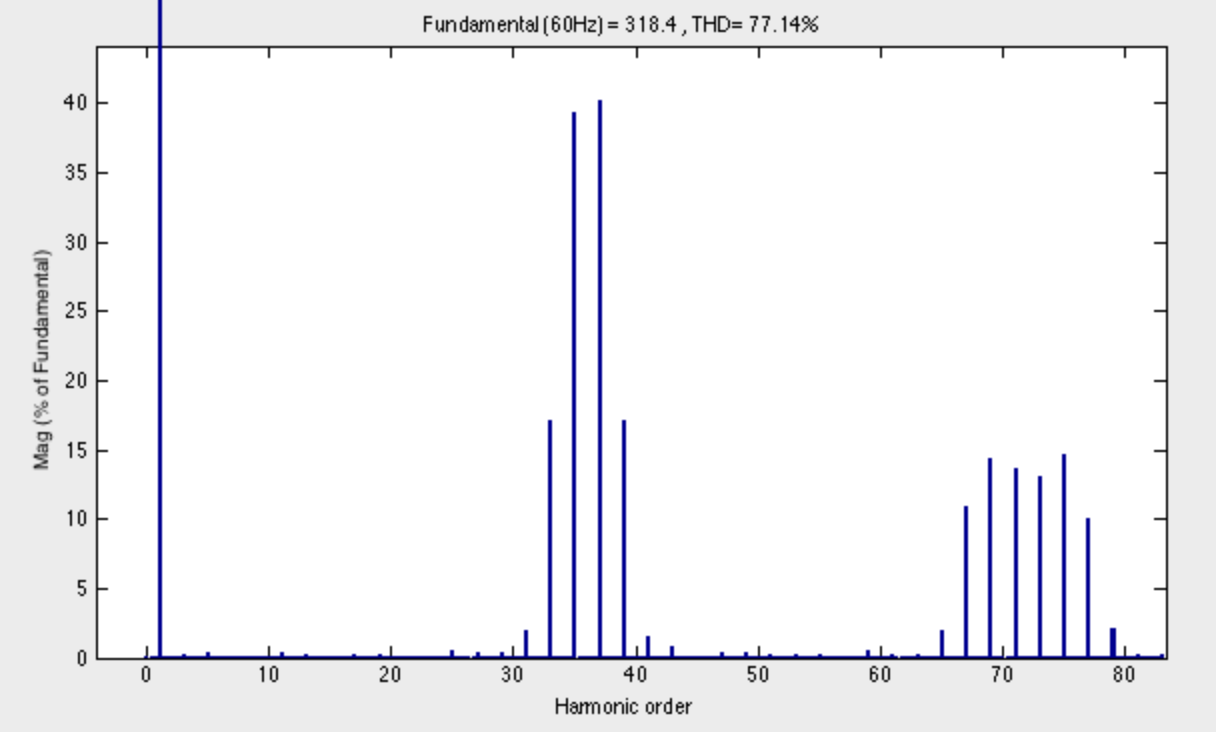
\includegraphics[width = 3.5in]{unipolarFFTMatlab}
\caption{The spectral content of a unipolar inverter is given by FFT, with harmonics shown as multiples of the fundamental at 60Hz}
\label{unipolarFFTMatlab}
\end{figure}

As for the bipolar case, the Fourier coefficients for the unipolar case are found to be:
\begin{equation}
a_n = \frac{2}{\pi} \Big[\int_{\theta_1}^{\theta_2} \cos(n\omega t) d\omega t + \int_{\theta_3}^{\theta_4} \cos(n\omega t)d\omega t +\ldots +
\int_{\theta_{2k-1}}^{\theta_{2k}} \cos(n\omega t)d\omega \Big]
\end{equation} 
and 
\begin{equation}
b_n = \frac{2}{\pi} \Big[\int_{\theta_1}^{\theta_2} \sin(n\omega t) d\omega t + \int_{\theta_3}^{\theta_4} -\sin(n\omega t)d\omega t +\ldots +
\int_{\theta_{2k-1}}^{\theta_{2k}} (-1)^k \sin(n\omega t)d\omega t \Big]
\end{equation} 

\subsection{Analyzing the Spectrum of the Hybrid PWM}
The results obtained for the hybrid PWM are thought to be quite similar to those of the bipolar switching scheme, due to the fact that they both allow switching directly from $+V_{dc}$ to $-V_{dc}$. Therefore, it can be safely assumed that both EMI and THD in the hybrid switching case will be unfavorable in comparison to the unipolar switching scheme.

\begin{figure}[ht]
\centering
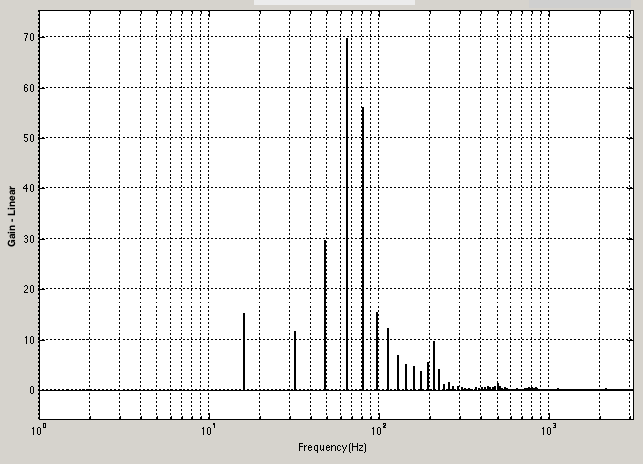
\includegraphics[width = 5in, height = 2in]{hybridSpectra}
\caption{The spectrum of the hybrid inverter, calculated from the voltage vector generated by the hybrid simulation. The output shows significant low frequency content with harmonics bunched around the fundamental.}
\label{hybridSpectra}
\end{figure}

The spectrum shown in Figure \ref{hybridSpectra} is rich in sub-fundamental content, with a much tighter bunching of harmonics around the fundamental as compared to other switching schemes studied thus far.

From an efficiency standpoint, it appears that the hybrid switching scheme is also at a disadvantage compared to unipolar due to the fact that the sine wave is traced out of a wave rapidly switching between $+V_{dc}$ to $-V_{dc}$ to obtain a sine wave, and hence we are `undoing' some of the peak voltage seen at the output. The result is lower $V_{rms}$ output from the bipolar switching, necessitating a higher voltage input. This voltage differential must be accounted for either by higher duty cycles of the boost converter, or more solar panels. While it would be a stretch to say that the boost converter is inefficient, the DC/DC stage is far from ideal, accounting for a large percentage of loss in inverters that utilize them. 

\begin{figure}[h]
\centering
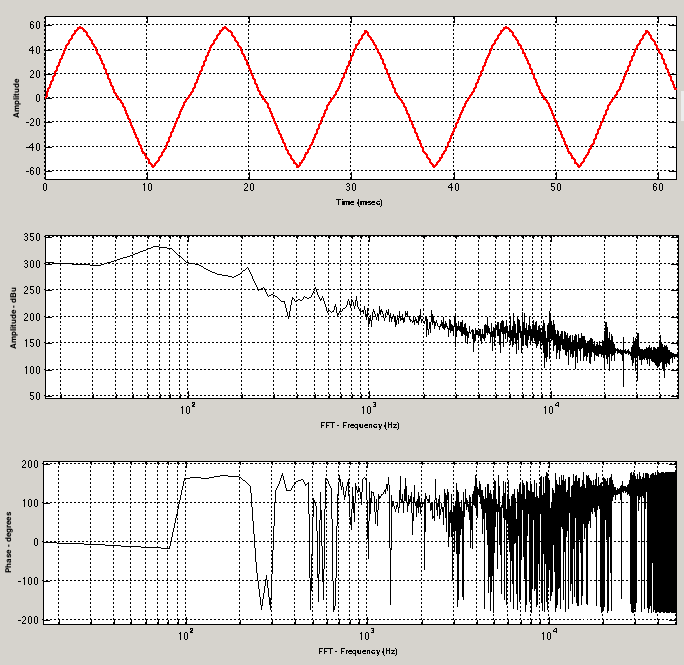
\includegraphics[width = 5.5in]{hybridFFT}
\caption{A plot showing voltage output of the hybrid inverter simulated in Matlab, as well as Fourier data for the magnitude (dB) and phase (degrees) respectively.}
\label{hybridFFT}
\end{figure}

From Figure \ref{hybridFFT}, we see that Bode plot of the voltage FFT confirms the presence of low frequencies at the output, with approximately $100dB$ per decade roll-off past the $60Hz$ cutoff. 

\subsection{Distortion in the Power Grid}
Power quality for the grid is subject to strict regulations that mandate either $60 Hz$ or $50 Hz$ operation depending on region. Grid-connected equipment and most consumer loads are designed for a set frequency. Deviation from these frequencies can result in serious system wide consequences including inefficiencies, interference and blackouts in the worst cases. Superimposed effects from variations in generation and loading conditions cause undesirable drift in the fundamental signal across the grid. An example of this is the spectral distortion caused by the nonlinear currents drawn by switching loads found in many consumer electronics and modern lighting ballasts. For comparison purposes, with the inverter discussed in this paper, the quality of the local power grid is analyzed. A time domain graph of a power cycle in our laboratory is shown in ~\ref{gridWave} 

\begin{figure}
\centering
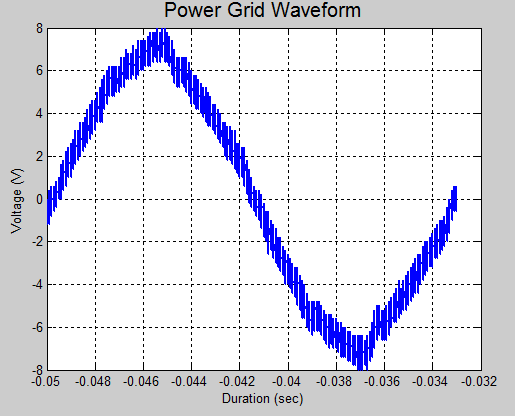
\includegraphics[width = 3.5in]{gridWave.png}
\caption{Power Grid Signal of the UC Santa Cruz Campus}
\label{gridWave}
\end{figure}

The ideal waveform for Figure ~\ref{gridWave} is a sinusoid but aspects of distortion are observable in the irregularities of the curve. The mean frequency during the test is $60.04 Hz$ with high and low values of $60.20 Hz$ and $59.90 Hz$ respectively. To better understand the non-ideal underlying signals causing these effects, a fast Fourier transform is taken on the grid wave to reveal its harmonic contents as shown in ~\ref{gridFFT}.

\begin{figure}
\centering
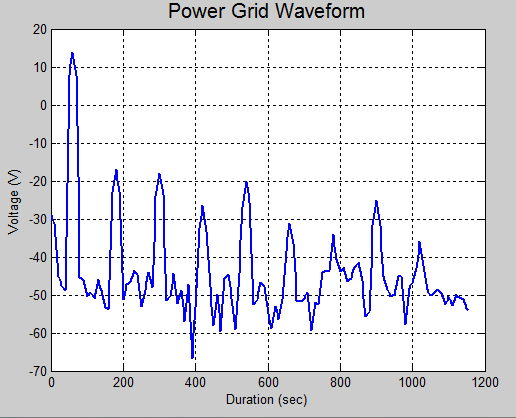
\includegraphics[width = 3.5in]{gridFFT.png}
\caption{Fast Fourier Transform Spectrum of UC Santa Cruz's Grid}
\label{gridFFT}
\end{figure}

The strength of the fundamental signal is apparent in Figure ~\ref{gridFFT} but the presence of harmonics is also seen. The odd order harmonics ($180 Hz$,$300 Hz$, ect.) in  Figure ~\ref{gridFFT} dominate the spectrum while even orders tend to have lesser influence due to their canceling nature. The total harmonic distortion is calculated to be $0.4\%$. These potentially harmful distortions are why preventative measures such as filtering and financial penalties are used for keeping grid-tied equipment within compliance. As the diversity of the grid grows, including the spread of distributed generation through photovoltaics, we must be aware of the quality of our electricity as it is important for a reliable grid.

\section{PWM Performance}
The reality of being a two-man team has definitely caught up with our lofty research ambitions on this project: to build and control a DC/DC boost circuit at output voltages in excess of $180V$; to build an inverter from the ground up and implement previously unimplemented controllers; and lastly, to characterize the THD, efficiency and robustness of the various inverter switching schemes.

If time were on our side, it would have been our wish to have implemented both bipolar and unipolar PWM in addition to hybrid PWM in order to compare their real world performance in terms of THD, efficiency, and robustness to disturbance; however, these analyses are what Masters theses are made of. With our limited time and budget, we were able to bounce back from a problematic Rev 1 board and send out a Rev 2 design in just a few days. Even still, the PCB turn times that were within our budget left us with all of a day and a half to power up and debug our hardware before our final presentation. 


In spite of the setbacks, and the impossible time-frame of a complete PCB overhaul, the Hybrid Inverter Team (HIT) is proud to present the 'HIT Power Conversion Development Board Rev. 2' to CITRIS and the Hybrid Systems Lab. With this tool, we have enabled the study of power conversion algorithms at the micro inverter scale. As an incoming graduate student to the Hybrid Systems Lab at UCSC, Ryan Rodriguez and Jun Chai plan on using this robust and extensible validation tool to perform more in-depth research on power conversion and the 'smart grid.' 

Our goal was to undertake a comparative study of the three PWM techniques that have been the focus of much of this work: bipolar or unipolar PWM, and the hybrid PWM. 
Due to severe time constraints, we have only had the opportunity to successfully demonstrate unipolar PWM operation on our custom hardware. With the successful results given below, we are confident that full operation of the hybrid algorithm is simply a matter of debugging time that we just do not have at the moment.


In the following section we discuss how the unipolar PWM technique fairs in our real-world tests on the HIT development board. These results are obtained using the FFT functionality of a Tektronix DPO 3054 oscilloscope, and are intended to verify the results we have obtained numerically in Section \ref{uniSection}. We also present fundamental results obtained from our outdoor test using the $170W$ Sharp PV module.

\subsection{Bipolar PWM}
In progress \ldots

\subsection{Unipolar PWM}
The Hybrid Inverter Team's board is characterized while running unipolar PWM with a focus on spectral output. FFT is implemented on the AC output of the inverter during experimental testing in lab while using a high power DC supply for system input. The test's resulting frequency spectrum is shown in Figure ~\ref{FFT HIT Board PWM After Filter}.

\begin{figure}
\centering
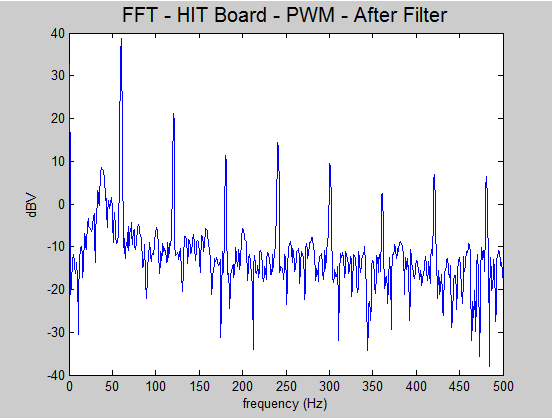
\includegraphics[width = 3.5in]{FFT_HIT_Board_PWM_After_Filter.PNG}
\caption{Frequency Spectrum of HIT Board Using Unipolar PWM}
\label{FFT HIT Board PWM After Filter}
\end{figure}

Figure ~\ref{FFT HIT Board PWM After Filter} depicts a fundamental signal at $60 Hz$ which dominates above the adjacent harmonics as seen by the logarithmic scale. The total harmonic distortion of this inverter output is calculated to be $19.84\%$ which is less than the $77.14\%$ predicted by the SimPower System's simulation. The lower THD value is likely a consequence of our test using a low pass filter on the inverter output to reduce higher frequency distortions.  These results still verify the presence of moderately significant distortion which is less than ideal in a power supply. 

In addition to the laboratory testing, an outdoor field test is conducted with a single PV panel and the HIT board operating with unipolar PWM. The experiment environmental conditions are close to optimal with a clear sky during mid-day in June. These conditions contribute to a high solar irradiance on the solar panel and allow for close to the maximum power draw. A resistive load is varied to alter current draw from the panel while input and output power measurements are taken. With no load, the open circuit voltage for the panel is resting at $40.1V$ which indicates the net effects of shunt diode currents in the solar cell network. The changing resistive load causes the terminal voltage of the panel to vary as expected from the non-linear IV loading curve. A minimum load of $100\Omega$ is placed on the $120VAC~ rms$ output of the inverter and a power output of $137W$ is achieved. Due to some suspected discrepancy in the current transformer clamp measurement tool used in the experiment, inverter board efficiency is approximately estimated to be about $80\%$ which correlates with the testing done on the boost converter. This indicates that upwards of $164W$ is sourced from the panel out of its capability of $170W$. The outdoor test setup at the Baskin School of Engineering is displayed in Figure ~\ref{Solar Test Setup}.

\begin{figure}
\centering
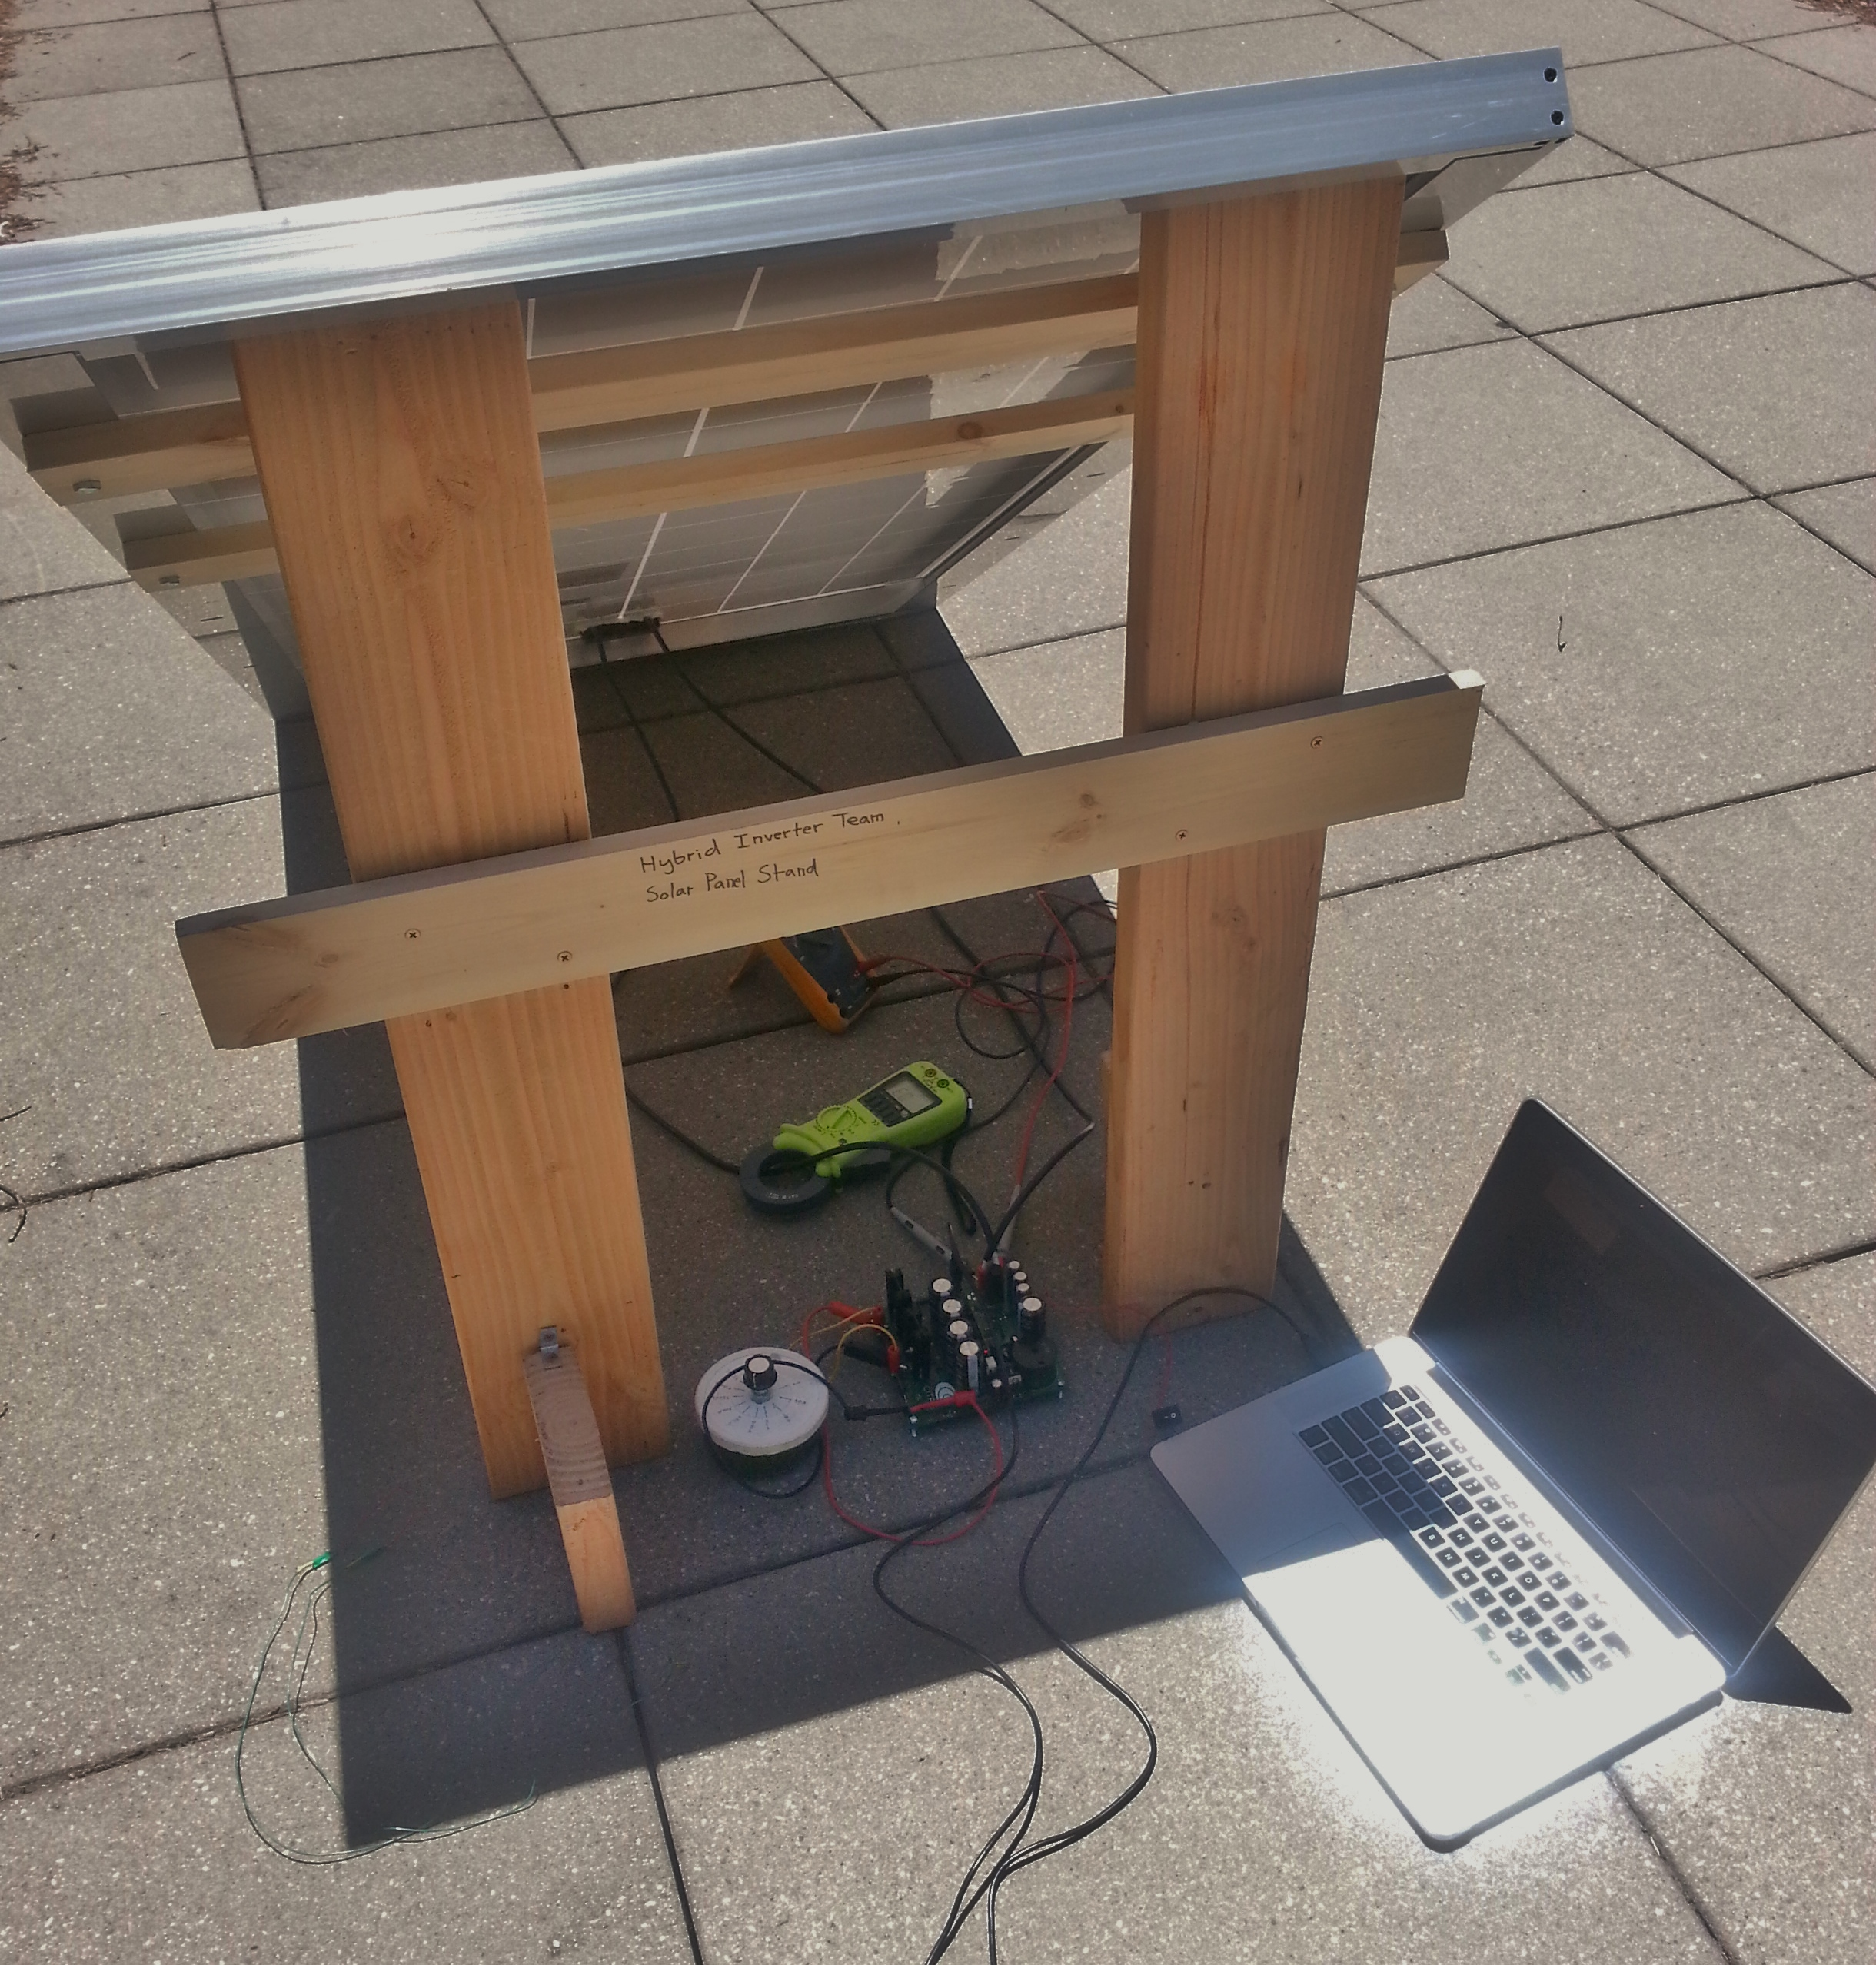
\includegraphics[width = 3.5in]{Solar_Test.jpg}
\caption{Outdoor HIT Board Solar Test Setup}
\label{Solar Test Setup}
\end{figure}
  
\subsection{Hybrid Performance}
In progress \ldots

\section{Conclusion}
Power conversion is far and above the most difficult task that a power systems designer working in the field of renewables can undertake due to the breadth that these engineers must possess; they need to have superior circuit analysis skills, a knack for using industry standard simulations tools, and a deft way with modern programming languages and digital signal controllers. Lacking any one of the above, it is nearly impossible to innovate, or even survive, in this space. The problems found in `standard' power converters are compounded in renewable energy systems where loading and sourcing conditions can fluctuate wildly throughout the course of any given day. With the demand for clean energy more dire than ever, engineers must push their understanding to squeeze every last Joule that their system can provide.

This study, motivated by the need for new and innovative conversion techniques, has sought to assess the viability of a new hybrid technique for PWM generation. We have attempted to cover many of the challenges encountered by power systems designers while planning the architecture of their power converters while addressing the most pressing concerns: harmonic content, efficiency, robustness, and ease of implementation.

Over the course of our 20+ week senior design project, we have come to understand the pulse-width modulation techniques that drive today's power converters, namely the single-phase inverter. The contender? A new hybrid technique for generating PWM signals. The reigning champion? The unipolar PWM technique. Although initial numerical results had shown that the new hybrid PWM technique was capable of producing a spectrum that was largely free from the low frequency content in the traditional PWM technique, it was later found that these simulations were taken from a simulation with a step disturbance at the input. It is believed that this disturbance contributed to the low frequency content found in the traditional PWM inverter. Additionally, it is a fundamental fact that the new hybrid technique is a closed lop system attempting to stabilize a state vector composed of current and voltage simultaneously. This system was compared to an open-loop bipolar PWM controller incapable of responding to a step response. Indeed, it has been stated in this research that closed-loop bipolar or unipolar PWM converters require PI or PID controllers to adjust duty cycle depending on the load or sourcing conditions at any given time. 